\documentclass[a4paper]{article}
\usepackage[utf8]{inputenc}
\usepackage{caption}
\usepackage{subcaption}
\usepackage[spanish]{babel}
\usepackage{graphicx}
\usepackage{xcolor}
\usepackage{amsmath}
\usepackage{hyperref}
\usepackage{todonotes}
\usepackage{biblatex}

\newcommand\imgScale {0.6}

\addbibresource{biblio.bib}

\title{Proyecto visión avanzada}
\author{Raúl Candela Arias \\ Francisco Morillas Espejo}
\date{Abril 2021}

\begin{document}

\maketitle

\section{Introducción}

El objetivo de este proyecto es el entrenamiento de redes convolucionales para realizar \textbf{segmentación semántica} de imágenes para detectar hasta \todo[fancyline]{revisar numero de clases}3 clases diferentes.
\newline

La segmentación semántica consiste en, dada una imagen, identificar a que clase de elemento corresponde cada píxel de esta.
Para ello, se crea una máscara de las mismas dimensiones que la imagen de entrada donde previamente se han coloreado las distintas clases (objetos) que se desean identificar (figura~\ref{fig:semanticSeg}).
\newline

La imagen original y la máscara se relacionan tal que, sea $A$ la imagen de entrada y $M$ la máscara, para cada píxel de la imagen $A_{i,j}$ tenemos que $M_{i,j} = c(A,i,j)$, donde $c$ es una función que indica a que clase pertenece el píxel ubicado en la imagen $A$ en la posición $i,j$.
\begin{figure}[htbp]
    \centering
    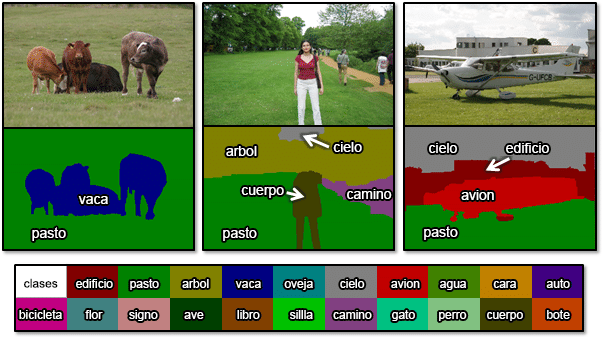
\includegraphics[scale=\imgScale]{img/EjSegSem.png}
    \caption{\small Ejemplo de segmentación semántica. \cite{Ref1}}
    \label{fig:semanticSeg}
\end{figure}

\section{Estado del arte}
A lo largo de la literatura se encuentran diferentes métodos para el reconocimiento de objetos a nivel de píxel, todos ellos haciendo uso de \textit{machine learning}~\cite{fabaret, long} pero, al unir series de convoluciones junto con capas de \textit{max-pooling} plantean problemas en la recreaci\'on de la imagen.
\newline

Por ello, Bradrinarayanan et al.~\cite{encoderDecoder} plantean una aproximaci\'on basada en arquitectura \textit{encoder-decoder}, solventando este problema y con unos resultados considerablemente superiores al resto.
En la figura~\ref{fig:segnet} se puede observar la arquitectura planteada.
\newline

Plantean una estructura en la que las capas del encoder y del decoder son sim\'etricas.
Las operaciones de \textit{upsamplig} del dedcoder usan los \'indices de la capa correspondiente de \textit{max-pooling} del encoder.
No hacen uso de conexiones residuales~\cite{resnet}.
\newline

Otra aproximaci\'on al problema es la planteada por Ronneberger et al.~\cite{unet} donde plantean una arquitectura encoder-decoder llamada UNet (figura~\ref{fig:unet} en la que mediante salto de conexiones o conexiones residuales se concatena la \'ultima capa de convoluci\'on de la parte del encoder con la primera capa de su correspondiente deconvoluci\'on en el decoder, generando una forma de u.
Por su forma la parte del encoder y del decoder son sim\'etricas.
\newline

Como red de base a las arquitecturas mencionadas previamente en ocasiones se emplean modelos de redes ya existentes y pre-entrenados para grandes conjuntos de datos como ImageNet~\cite{imagenet} o COCO~\cite{coco}.
Entre estas se pueden destacar algunas como ResNet~\cite{resnet}, Xception~\cite{xception} o VGG-16~\cite{vgg} que destacan entre las m\'as comunes.

%A partir de esta idea, el modelo ded \textit{encoder-decoder} es el empleado en este campo de la visi\'on artificial.
%Aunque se distinguen diferentes arquitecturas para las dos partes.
%Dentro de las diferentes aproximaciones para la tarea de clasificación semántica se encuentra el modelo de \textit{encoder-decoder} como el más empleado.
%\newline

%En este tipo de modelos se recibe la imagen original como entrada y se pasa por una serie de capas convolucionales para extraer sus características aunque, como consecuencia la imagen reduce su tamaño.
%Tras esto se pasa por una serie de capas de deconvolución cuya salida proporcionará la máscara semántica de la imagen en cuestión.

\section{Desarrollo}
\todo{completar}
Para la implementación de la red se ha empleado una arquitectura \textit{UNet} basada en el modelo \textit{Xception} mediante la creaci\'on de una subclase de tipo \texttt{Model} dentro de la API de \texttt{Keras}.
\newline

La arquitectura presenta un modelo encoder-decoder con cuatro tama\~nos de filtros diferentes, 32, 64, 128 y 256, tanto para las capas convolucionales como para las deconvoluciones.

\section{Problemas encontrados}
\subsection{Creación la clase UNetX}
A la hora de crear el modelo se optó por realizarlo heredando de la clase \texttt{Model} de la API de \texttt{Keras}, lo cual ocasionó problemas debido a la falta de ejemplos de redes convolucionales complejas realizadas de este modo.
\newline

Una vez solventado, el m\'etodo de generar el modelo mediante herencia proporciona una mayor flexibilidad en cuanto al tipo de conexiones a realizar entre las capas, la posibilidad de generar diferentes modelos con distintos filtros o con una entrada de diferente tama\~no a lo largo del c\'odigo sin tener que crear nuevas funciones para cada caso.


\subsection{Carga del dataset \textit{Semantic Drone}}
A la hora de realizar la carga del dataset hubieron varios problemas, entre ellos el formato de carga de las imágenes, la necesidad de procesar las etiquetas y la velocidad de carga de estas.\newline

En cuanto al formato, se empezó cargándolas con \textit{OpenCV} y reescal\'andolas a un tamaño de 480p, pero las imágenes eran demasiado grandes y finalmente se optó por realizar la carga con un tamaño de 224x224.\newline

Con respecto al procesado de las etiquetas, estas venían en formato \textit{.png} y debían ser reescaladas al mismo tamaño que la imagen original y convertirlas de una imagen con 3 canales a una matriz con las id de las etiquetas en cada píxel. Esta última conversión era excesivamente lenta y se intentó tanto realizarla en C como utilizar \texttt{numba} para intentar acelerarlo. Siendo esta la opción definitiva escogida.\newline

Finalmente se optó por utilizar el formato de imágenes de \texttt{PIL} y cargarlas con los métodos de \texttt{keras.preprocessing.image}.

\section{Resultados}
\todo{hacer todo}

\section{Conclusiones}
\todo{hacer todo}

\newpage
\printbibliography
\end{document}
